%  !TeX  root  =  user_guide.tex

\chapter{Premiers Pas}\label{label_getstarted}

% when the revision of a section has been finalized, 
% comment out the following line:
% \updatedisclaimer

%This chapter gives a quick overview of installing QGIS, some sample 
%data from the QGIS web page and running a first and simple session 
%visualizing raster and vector layers.

Ce chapitre donne un bref aperçu de l'installation de \qg, de quelques jeux de données provenant du site Internet et du lancement d'une première session d'affichage de couches matricielles et vectorielles.

\section{Installation}\label{label_installation}
\index{installation}

%Installation of QGIS is very simple. Standard installer packages are
%available for MS Windows and Mac OS X. For many flavors of GNU/Linux binary packages (rpm and deb) or software repositories to add to your %installation manager are provided. Get the latest information on binary packages at the QGIS website at \url{http://qgis.osgeo.org/download/}.

L'installation de \qg est très simple, des installateurs sont disponibles pour les systèmes d'exploitation \mswin et \mac. Beaucoup de distributions \tux mettent à disposition des fichiers binaires précompilés (.rpm ou .deb) ou des dépôts sources via leurs interfaces de gestion de logiciels. Vous pouvez obtenir les dernières informations concernant les paquets binaires sur le site de \qg sur \url{http://qgis.osgeo.org/download/}.

%\minisec{Installation from source}

%If you need to build QGIS from source, please refer to the coding and
%compiling guide available at \url{http://qgis.osgeo.org/documentation/}. 
%The installation instructions are also distributed with the QGIS source
%code.

\minisec{Installation à partir des sources}

Si vous désirez installer \qg à  partir des sources, veuillez vous référer au guide de codification et de compilation disponible sur \url{http://qgis.osgeo.org/documentation/}.
Les instructions d'installation sont également diffusées avec le code source de \qg.

\section{Échantillon des données}\label{label_sampledata}
\index{Échantillon des données} 

%The user guide contains examples based on the QGIS sample dataset. 
%\win The Windows installer has an option to download the QGIS sample dataset.
%If checked, the data will be downloaded to your \filename{My Documents}
%You may use Windows Explorer to move this folder to any convenient location.
%If you did not select the checkbox to install the sample dataset
%during the initial QGIS installation, you can either
%\begin{itemize}
%\item use GIS data that you already have;
%\item download the sample data from the QGIS website
% \url{http://qgis.osgeo.org/download}; or
%\item uninstall QGIS and reinstall with the data download option checked, only if 
%the above solutions are unsuccessful.
%\end{itemize}

Le guide d'utilisateur contient des exemples basés sur l'échantillon du jeu de données inclus dans \qg.
\par
\win L'installateur \mswin possède une option qui permet de télécharger l'échantillon du jeu de données \qg.
Si vous le cochez, les données seront téléchargées dans votre répertoire intitulé \filename{Mes Documents} et placées dans le répertoire \filename{GIS Database}. Vous pouvez utiliser l'explorateur \mswin pour vous déplacer à partir de ce répertoire vers d'autres répertoires de votre choix.
Si vous ne cochez pas cette option durant l'installation, vous avez plusieurs solutions:
\begin{itemize}[label=--]
\item utilisez les données que vous possédez déjà;
\item télécharger l'échantillon sur le site de \qg
 \url{http://qgis.osgeo.org/download}; ou
 \item désinstaller et réinstaller \qg en cochant la case de téléchargement.
\end{itemize}
\par\bigskip
%\nix \osx For GNU/Linux and Mac OSX there are not yet dataset installation
%packages available as rpm, deb or dmg. To use the sample dataset download the
%file \filename{qgis\_sample\_data} as ZIP or TAR archive from
%\url{http://download.osgeo.org/qgis/data/} and unzip or untar the archive on
%your system. The Alaska dataset includes all GIS data that are used as
%examples and screenshots in the user guide, and also includes a small \grass
%database. The projection for the QGIS sample dataset is Alaska Albers Equal
%Area with unit feet. The EPSG code is 2964.

\nix \osx Pour les systèmes \tux et \mac il n'y a pas encore de paquets disponibles sous forme de rpm, deb ou dmg. Pour utiliser l'échantillon de données, téléchargez le fichier compressé au format ZIP ou archive TAR \url{http://download.osgeo.org/qgis/data/}
à partir du lien \url{http://download.osgeo.org/qgis/data/} et décompressez-le dans votre système. Le jeu de données sur l'Alaska comporte toutes les données SIG qui ont servi à la préparation des captures d'écran et des exemples qui figurent dans ce manuel. La projection est l'Alaska Albers Equal Area qui a pour unité le pied et dont le code EPSG est le 2964.
\par
\begin{verbatim}
PROJCS["Albers Equal Area",
    GEOGCS["NAD27",
        DATUM["North_American_Datum_1927",
            SPHEROID["Clarke 1866",6378206.4,294.978698213898,
                AUTHORITY["EPSG","7008"]],
            TOWGS84[-3,142,183,0,0,0,0],
            AUTHORITY["EPSG","6267"]],
        PRIMEM["Greenwich",0,
            AUTHORITY["EPSG","8901"]],
        UNIT["degree",0.0174532925199433,
            AUTHORITY["EPSG","9108"]],
        AUTHORITY["EPSG","4267"]],
    PROJECTION["Albers_Conic_Equal_Area"],
    PARAMETER["standard_parallel_1",55],
    PARAMETER["standard_parallel_2",65],
    PARAMETER["latitude_of_center",50],
    PARAMETER["longitude_of_center",-154],
    PARAMETER["false_easting",0],
    PARAMETER["false_northing",0],
    UNIT["us_survey_feet",0.3048006096012192]]
\end{verbatim}

%If you intend to use QGIS as graphical frontend for \grass, you can find a
%selection of sample locations (e.g. Spearfish or South Dakota) at the
%official \grass GIS website \\
%\url{http://\grass.osgeo.org/download/data.php}. 

Si vous désirez utiliser \qg comme une interface à \grass, vous trouverez une sélection d'échantillons de secteur (e.g. Spearfish ou South Dakota) sur le site officiel de \grass \\
\url{http://grass.osgeo.org/download/data.php}. 

%\subsection{Sample Session}\label{samplesession}

%Now that you have QGIS installed and a sample dataset available, we would 
%like to demonstrate a short and simple QGIS sample session. We will visualize 
%a raster and a vector layer. We will use the landcover raster 
%layer \filename{qgis\_sample\_data/raster/landcover.img} and the lakes 
%vector layer \filename{qgis\_sample\_data/gml/lakes.gml}.

\section{Étape pratique}\label{samplesession}

Maintenant que vous avez \qg d'installé avec un échantillon de données disponibles, nous aimerions vous faire une courte démonstration. Vous allez visualiser une couche raster et une couche vecteur.

Nous allons utiliser la couche raster landcover \filename{qgis\_sample\_data/raster/landcover.img} 
et la couche vectorielle des lacs \filename{qgis\_sample\_data/gml/lakes.gml}.


%\minisec{start QGIS}

%\begin{itemize}
%\item \nix{Start QGIS by typing: \usertext{qgis} at a command prompt, or
%if using precompiled binary, using the Applications menu.}
%\item \win{Start QGIS using the Start menu or desktop shortcut, 
%or double click on a QGIS project file.}
%\item \osx{Double click the icon in your Applications folder.}
%\end{itemize} 

%\begin{figure}[ht]
   %\begin{center}
   %\caption{A Simple QGIS Session \nixcaption}\label{fig:simple_session}\smallskip
   %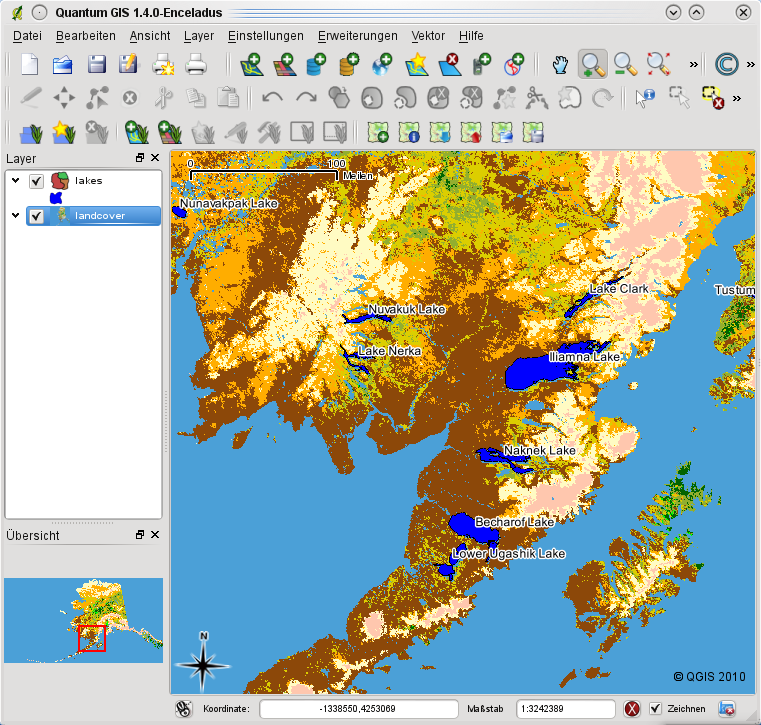
\includegraphics[clip=true, width=12cm]{simple_session}
%\end{center}
%\end{figure}

\minisec{Démarrer \qg}

\begin{itemize}[label=--]
\item \nix{Démarrer \qg en tapant: \usertext{qgis} en ligne de commande dans une console, ou
en cliquant tout simplement sur le fichier binaire pré-compilé, du menu Application.}
\item \win{Démarrer \qg en utilisant le menu Démarrer ou un raccourci sur placé sur le Bureau, 
ou double-cliquez sur un fichier de projet existant de \qg.}
\item \osx{Double-cliquez sur l'icône de \qg dans votre répertoire du menu Applications.}
\end{itemize} 

\begin{figure}[ht]
   \begin{center} 
   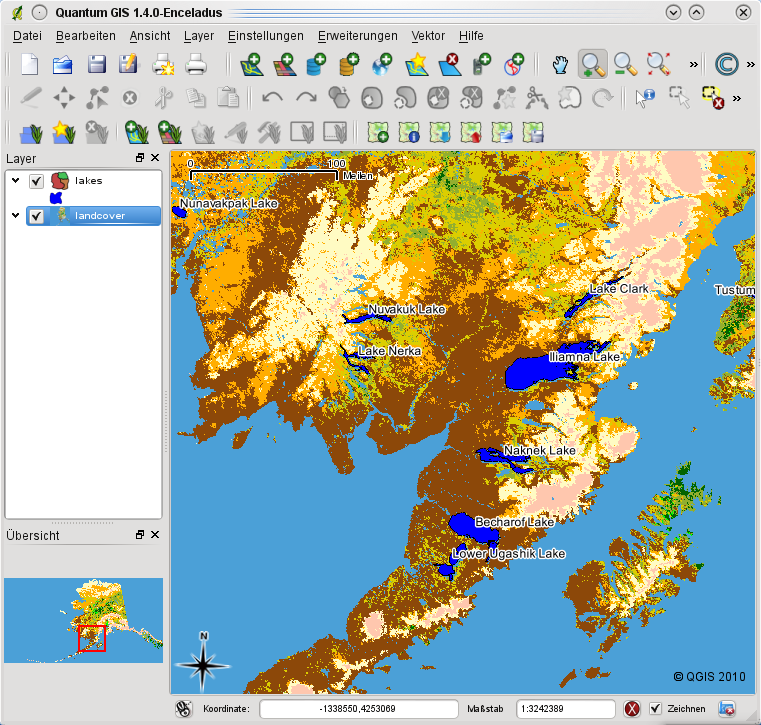
\includegraphics[clip=true, width=12cm]{simple_session}
   \caption{Une session de \qg  \nixcaption}\label{fig:simple_session}
\end{center}
\end{figure}


%\minisec{Load raster and vector layers from the sample dataset}

%\begin{enumerate}
%\item Click on the \toolbtntwo{mActionAddRasterLayer}{Load Raster} icon.
%\item Browse to the folder \filename{qgis\_sample\_data/raster/}, select 
%the ERDAS Img file \filename{landcover.img} and click \button{Open}.
%\item If the file is not listed, check if the Filetype combobox at the
%bottom of the dialog is set on the right type, in this case "Erdas Imagine
%Images (*.img, *.IMG)"
%\item Now click on the \toolbtntwo{mActionAddOgrLayer}{Load Vector} icon. 
%\item \radiobuttonon{'File'} should be selected as Source Type in the new
%\dialog{Add Vector Layer} dialog. Now click \button{Browse} to select the
%vector layer.
%\item Browse to the folder \filename{qgis\_sample\_data/gml/}, select "GML"
%from the filetype combobox, then select the GML file \filename{lakes.gml} 
%and click \button{Open}, then in Add Vector dialog click \button{OK}.
%\item Zoom in a bit to your favorite area with some lakes.
%\item Double click the \filename{lakes} layer in the map legend to open the 
%\dialog{Layer Properties} dialog.
%\item Click on the \tab{Symbology} tab and select a blue as fill color.
%\item Click on the \tab{Labels} tab and check the \checkbox{Display labels} 
%checkbox to enable labeling. Choose NAMES field as Field containing label.
%\item To improve readability of labels, you can add a white buffer around them,
%by clicking ``Buffer'' in the list on the left, checking \checkbox{Buffer
%labels?} and choosing 3 as buffer size.
%\item Click \button{Apply}, check if the result looks good and finally
%click \button{OK}.
%\end{enumerate} 

%You can see how easy it is to visualize raster and vector layers in 
%QGIS. Let's move on to the sections that follow to learn more about the 
%&available functionality, features and settings and how to use them.


\minisec{Charger les couches raster et vecteur depuis le jeu de données}
{\setlength{\baselineskip}{1.3\baselineskip}
\begin{enumerate}[itemsep=2pt]
\item Cliquez sur l'icône \toolbtntwo{mActionAddRasterLayer}{Ajouter une couche Raster}.
\item Parcourez le dossier \filename{qgis\_sample\_data/raster/}, sélectionnez 
le fichier ERDAS Img\\
 \filename{landcover.img} et cliquez \button{Ouvrir}.
\item Si le fichier n'est pas listé, vérifiez le type de fichier à partir du menu déroulant 
au dessous de la boîte de dialogue afin de sélectionner le bon type de fichier, dans ce cas-ci c'est \selectstring{Fichiers de type}{Erdas Imagine (*.img, *.IMG)}
\item Maintenant cliquez sur l'icône \toolbtntwo{mActionAddOgrLayer}{Ajouter une couche vecteur}. 
\item \radiobuttonon{Fichier} devrait être sélectionné comme Type de source dans la nouvelle boîte de dialogue 
\dialog{Ajouter une couche vecteur}. Maintenant cliquez \button{Parcourir} pour sélectionner la couche vecteur
\item Parcourez le répertoire \filename{qgis\_sample\_data/gml/}, sélectionnez "GML"
à partir du menu déroulant Type de fichier, et sélectionnez ainsi le fichier GML \filename{lakes.gml} 
et cliquez sur \button{Ouvrir}, ensuite, dans la boîte de dialogue Ajouter une couche vecteur, cliquez \button{OK}.
\item Zoomez sur une zone de votre choix avec quelques lacs.
\item Double-cliquez la couche \filename{lakes} dans la liste des cartes pour ouvrir la fenêtre\\ \dialog{Propriété des couches}.
\item Cliquez sur l'onglet \tab{Convention des signes} et sélectionnez le bleu comme couleur de remplissage.
\item Cliquez sur l'onglet \tab{Étiquettes} et cochez la case \checkbox{Afficher les étiquettes} pour permettre l'étiquetage des attributs. 
Choisissez le champ contenant une étiquette comme champ d'étiquetage.
\item Pour améliorer la lisibilité des étiquettes, vous pouvez ajouter un halo atour d'eux,
en cliquant sur ``tampon'' dans la liste à gauche, cliquant \checkbox{Étiquettes tampon} et choisissez 3 comme taille du tampon.
\item Cliquez \button{Appliquez}, et vérifiez si le résultat est satisfaisant et enfin cliquez sur \button{OK}.
\end{enumerate} 
\par}
Vous pouvez constater combien il est facile d'afficher des couches rasters ou vecteur dans \qg.Passons aux sections suivantes pour apprendre plus sur les autres fonctionnalités, caractéristiques et paramètres disponibles et la façon de les utiliser.
